\title{\textbf{When Is the Vector Enough?\\
Frozen Residual Readouts versus Answer-Token Scoring}}
\ifdefined\AnonymousVersion
\author{Anonymous Author(s)}
\date{}
\else
\author{
  Hanan Herzog\\
  \texttt{hanan.herzog@gmail.com}
}
\date{}
\fi

\begin{document}
\maketitle

\begin{abstract}
When does a language model's frozen residual already support the answer, and
when does answer-token scoring add value? We compare a small supervised
classifier on final-token residual states with zero-/few-shot closed-set
answer-token scoring across six open-weight models on BoolQ, RuleTaker, and
ARC-Challenge. The methods use the same frozen backbone but different task
supervision and prompt lengths. Their relative performance is structured
rather than universal: the final-layer readout is numerically higher than
requested eight-shot scoring in five of six RuleTaker cases and two of six
BoolQ cases, whereas scoring is higher in all six ARC cases. On ARC the
scorer's advantage is ordered by readout competence across all six models,
falling from 10.6 points where the readout is weakest to under one point for
the two strongest readouts.

Existing small-budget refits qualify the result. Stored 64-label readouts
fall below the eight-shot scorer in 17 of 18 cells, and BoolQ
class-balanced refits do not preserve the full-training readout's advantage,
so that advantage is not established as supervision-independent. Intermediate
layer sweeps show that answer-relevant information is often accessible before
the final layer: in 12 of 18 cells the best swept layer exceeds the final one
by more than a crude selection-noise scale, although evaluation-selected
maxima still do not establish held-out gains or early exit. The scorer is the stored product-of-token-probabilities
heuristic, not marginalized answer likelihood or free-form generation. The
contribution is therefore a protocol-specific regime map: readouts are often
competitive on rule- and passage-grounded tasks, while scoring is most useful
when the residual readout is still weak.
\end{abstract}

\section{Introduction}

A frozen language model offers more than one interface for classification.
One can use its answer-token outputs, or train a separate classifier on its
internal representations. These interfaces need not give the same accuracy:
the output head was trained for next-token prediction, while a supervised
readout is fitted to the target task's labels. A useful empirical question is
how the two procedures compare under explicitly stated training and inference
budgets, rather than whether an answer is literally present in a vector.

We compare a one-hidden-layer MLP on final-token residual states with
zero-/few-shot answer-token scoring. Both use a frozen backbone and one prompt
forward pass per example, but they do not use identical prompts or equal
amounts of task-specific supervision. In the main experiments, the classifier
is fitted on thousands of labeled examples; the scorer receives a small
number of labeled demonstrations in its prompt. The scorer is allowed a
longer context, which can preserve more passage text and demonstrations but
does not compensate in a controlled way for the classifier's training labels.

Our contribution is a cross-model, cross-task map of when these two readouts
separate, together with a supervision-budget qualification and layerwise
readouts. This is not a supervision-matched superiority result or a test of
generated iterative reasoning. The main observations are:
\begin{enumerate}
\item \textbf{Scoring's value is regime-dependent.} The final-layer
classifier is numerically higher than the fixed eight-shot scorer in five
RuleTaker cases and two BoolQ cases, while the scorer is higher in all six
ARC cases. The largest scorer gaps occur where the readout is weakest: across
all six ARC models the gap falls monotonically with readout accuracy, apart
from a 0.4-point inversion between the two strongest readouts
(Table~\ref{tab:main}).
\item \textbf{Supervision changes the comparison.} Stored 64-label readouts
exist for all 18 cells and fall below the corresponding eight-shot scorer in
17 of them, including all six RuleTaker cells. On BoolQ, where matched
requested-shot arms exist, matching the number of classifier training labels
to the requested number of demonstrations does not preserve the
full-training classifier's advantage (Table~\ref{tab:budget}). These
artifacts match declared counts, not independently verified example
identities or retained prompt counts.
\item \textbf{Answer-relevant information is often accessible before the
final layer.} Several intermediate layers support higher readout accuracy
than the final layer, and in 12 of 18 cells by more than the scale of the
optimism that picking a maximum introduces. These evaluation-selected maxima
still do not establish held-out gains from layer selection or justify
stopping the backbone early (Table~\ref{tab:placement}).
\end{enumerate}

The interpretation is further limited by the implemented scoring heuristic:
its aggregation of alternative tokens differs from probability
marginalization. We describe the exact rule below and retain its measured
accuracies without presenting it as the strongest available output baseline.

\section{Setup and Method}
\label{sec:setup}

\subsection{Supervised residual readout}

Let $h_T\in\mathbb{R}^d$ denote the last nonpadding token's output from
the final transformer block of a frozen model, before subsequent model-level
normalization or output processing. For DeepSeek, grouped trailing output
dimensions are flattened into a feature vector, giving an effective input
width of 16384 (the other model widths range from 1024 to 4096). The readout
capacity is therefore not constant across models: at a fixed hidden width the
first layer holds 16 times as many parameters for DeepSeek as for
Qwen3-0.6B. DeepSeek has the highest readout accuracy on BoolQ and ARC, and
this asymmetry is a candidate explanation that the present runs do not
separate from backbone quality. The prompt includes the
question and, where supplied by the task, the passage. Gold answers are not
appended to the readout's input. Prompts are left-truncated to 384 tokens,
retaining the prompt suffix and trailing answer slot, but not necessarily
the complete question. We standardize features using training-set means and standard
deviations and fit a width-128, one-hidden-layer ReLU MLP. The implementation
uses full-batch Adam with learning rate $10^{-3}$ for 150 epochs, with binary
or multiclass cross-entropy as appropriate. The backbone is never updated;
the MLP is nevertheless a task-supervised model.

The main readout statistic is the mean accuracy over four training seeds,
with their standard deviation. It is neither the accuracy of the best seed
nor that of a seed-vote ensemble. Logistic-regression readouts and other
feature transformations are secondary analyses; selection of regularization
or projection dimension on evaluation accuracy is exploratory.

\subsection{Implemented answer-token scorer}
\label{sec:scorer}

The baseline processes a task prompt with zero or $k$ balanced demonstrations
from the training split. Demonstrations are selected in class round-robin
order from the shuffled training rows; selection is not averaged over
different exemplar sets or orders. The round-robin is deterministic and
cycles the classes in a fixed order, so for the binary tasks at even $k$ the
demonstration immediately preceding the query always carries the same label.
Few-shot predictions are known to be sensitive to exactly this kind of
exemplar order and label balance \citep{zhao2021calibrate}, and the stored
runs do not vary either. Both methods choose from the same closed
answer set: Yes/No for BoolQ and RuleTaker, and A--D for ARC. The baseline
does not generate intermediate reasoning or a free-form answer. The stored
artifacts and table columns name these arms \texttt{loop.zero} and
\texttt{loop.$k$} for historical reasons; we call them scorer arms
throughout.

For each answer class $c$, the implementation constructs a token-ID set
$S_c$ from bare and space-prefixed answer variants tokenized after
\texttt{Answer:}. It slices off the number of tokens in the standalone
prefix, unions the remaining IDs, and removes IDs shared by classes.
At the last prompt token, it computes
\begin{equation}
s_c(x)=\sum_{t\in S_c}\log p_\theta(t\mid x),\qquad
\hat{y}=\mathop{\mathrm{argmax}}_c s_c(x).
\end{equation}
Thus it ranks the \emph{product} of the individual token probabilities, not
the sum of probability mass for mutually exclusive answer variants.
Marginalization over single-token alternatives would instead use
$\log\sum_{t\in S_c}p_\theta(t\mid x)$. Collecting IDs from a multi-token
variant also does not compute that variant's sequence likelihood.

A local tokenizer audit found two IDs per Yes/No class for each of the six
model tokenizers. On ARC, Mistral and Granite have two IDs per class; the
Qwen and DeepSeek tokenizers yield one retained ID per class. In the latter
cases, bare letter variants change the prefix tokenization and contribute
no suffix IDs under the implemented slicing rule. Consequently, even where
sum and marginalization coincide for the retained singleton, the procedure
does not establish coverage of all intended answer variants.

All reported scorer accuracies use this existing heuristic. Its numerical
difference from a corrected scorer is unmeasured. The pipeline saves
aggregate accuracies and, on fresh runs, class predictions rather than the
token probabilities needed to rescore offline. These results should not be
read as comparisons against standard answer-likelihood scoring generally.
None of the standard corrections to closed-set answer scoring are applied
here; \S\ref{sec:related} collects them. Token-level decision rules of this
kind are known to be suboptimal relative to hidden-state criteria on the same
frozen model \citep{cho2025hidden}, so our scorer is a weak rather than a
strong output baseline, and the readout-favorable cells below are the ones to
treat with most caution.

\subsection{Supervision, context, and reporting}

The main readouts use 9427 training labels on BoolQ, 10000 on RuleTaker,
and 1000 on ARC. The ARC filter leaves 1117 four-choice training rows and
1165 test rows; the reported training set is a seed-0 subsample of 1000 rows.
We report zero- and eight-shot scorer arms separately,
without selecting the stronger arm for the main comparison. This is a
reporting choice for the present descriptive analysis, not a preregistered
experimental design. Additional BoolQ runs requested up to 64 demonstrations.

The scorer's token cap is 8192 for Qwen BoolQ runs and 2048
otherwise, compared with the readout's 384. Left truncation can remove
passage content, complete demonstrations, or parts of demonstrations. The
stored results do not measure per-row truncation or the number of retained
complete demonstrations. We therefore use \emph{requested shots}, not
effective shots. Equal question identities and answer sets do not imply
equal token-level inputs or supervision.

Table~\ref{tab:main} reports seed means and SDs for the classifier and single
accuracies for the scorer. SD describes training-seed variation on the fixed
evaluation set, not a confidence interval for population performance.
Historical paired tests used separately fitted four-seed vote predictions;
they do not directly test the displayed seed-mean differences. We do not
attach those tests to the present descriptive tables. Small numerical
differences are not evidence of equivalence, and no count of significant
wins or corrected discoveries is claimed.

\subsection{Models and datasets}

The models are Qwen3-0.6B, Qwen3-4B, Qwen3-8B, Mistral-7B-v0.3,
Granite-3.1-8B-base, and DeepSeek-V4-Flash (the stored model slug is
\texttt{DeepSeek-V4-Flash-0731}). These are six models from four families,
including dense and mixture-of-experts architectures, not a controlled
architecture or parameter-count ablation.
Reported backbone runs use batch size 8; DeepSeek uses the local quantized
checkpoint loading path. Training-seed SD does not include variation from
backbone numerical execution.

BoolQ \citep{clark2019boolq} uses the \texttt{google/boolq} training split
and its 3270-row validation split. RuleTaker \citep{clark2020ruletaker}
uses \texttt{tasksource/ruletaker}, with 10000 sampled training rows and
4000 sampled rows from the official \emph{test} split. The artifacts call
the latter \texttt{val}; this is an evaluation-set name, not the official
validation split. ARC-Challenge \citep{clark2018arc} uses
\texttt{allenai/ai2\_arc}, retaining four-choice items, with 1117 filtered
training rows and 1165 test rows. The reported 1000-row training set is a
seed-0 subsample. No retrieval corpus is supplied for ARC, but the question
and choices themselves remain part of the input.

% Wide floats are declared next to the text that discusses them: four table*
% environments plus three full-width figures compete for a body of about ten
% pages, so declaring them in one block strands whichever group comes second.
% Generated by python3 scripts/build_descriptive_tables.py; do not edit numbers.
% Sources are explicit local results/*.json mappings in that stdlib-only script.
% Requires booktabs and graphicx. Input once before any table file.
\providecommand{\fittable}[1]{%
  \sbox0{#1}%
  \ifdim\wd0>\textwidth
    \resizebox{\textwidth}{!}{\usebox0}%
  \else
    \usebox0
  \fi
}

% Generated by python3 scripts/build_descriptive_tables.py; do not edit numbers.
% Sources are explicit local results/*.json mappings in that stdlib-only script.
\begin{table*}[t]
\centering
\caption{\textbf{Fixed final-layer readout and closed-set scorer accuracies}
(accuracy). Readout is the stored \texttt{last.mlp} mean $\pm$ seed SD
(four seeds; SD uses divisor four, not a confidence interval).
\texttt{loop.zero} and \texttt{loop.8} are the stored artifact keys for the
zero-shot and requested 8-shot scorer arms (\S\ref{sec:scorer}); they are
accuracies under the manuscript's product-of-token-probabilities heuristic,
not marginalized answer probabilities or free-form generation.
$\Delta=$ readout mean $-$ \texttt{loop.8}, with no baseline selection
or significance testing. Artifact-declared train/evaluation/loop counts:
BoolQ 9427/3270/3270; RuleTaker 10000/4000/4000;
ARC-Challenge 1000/1165/1165. BoolQ Mistral/Granite readouts use sweep
files and loops use full-evaluation reruns, not the sweeps' 405-row loops.
Readout token cap is 384; loop cap is 8192 for BoolQ Qwen and 2048
otherwise. These are different input and supervision protocols, not a
matched-label-budget comparison; requested demonstrations are not measured
retained counts.}
\label{tab:main}
\small
\setlength{\tabcolsep}{4pt}%
\fittable{%
\begin{tabular}{@{}llcccc@{}}
\toprule
Task & Model & Readout mean $\pm$ SD & \texttt{loop.zero} & \texttt{loop.8} & $\Delta$ vs.\ 8-shot \\
\midrule
% Readout: boolq_budget_06b.json; loops: boolq_budget_06b.json
BoolQ & Qwen3-0.6B & $0.746 \pm 0.004$ & 0.631 & 0.645 & $+0.101$ \\
% Readout: boolq_budget_4b.json; loops: boolq_budget_4b.json
 & Qwen3-4B & $0.856 \pm 0.002$ & 0.855 & 0.865 & $-0.009$ \\
% Readout: boolq_budget_8b.json; loops: boolq_budget_8b.json
 & Qwen3-8B & $0.878 \pm 0.002$ & 0.862 & 0.876 & $+0.001$ \\
% Readout: boolq_layersweep_mistral7b.json; loops: boolq_mistral7b_rerun.json
 & Mistral-7B & $0.841 \pm 0.002$ & 0.824 & 0.863 & $-0.022$ \\
% Readout: boolq_layersweep_granite8b.json; loops: boolq_granite8b_rerun.json
 & Granite-3.1-8B & $0.854 \pm 0.001$ & 0.800 & 0.865 & $-0.011$ \\
% Readout: boolq_layersweep_dsv4.json; loops: boolq_layersweep_dsv4.json
 & DeepSeek-V4-Flash & $0.896 \pm 0.001$ & 0.888 & 0.906 & $-0.009$ \\
\midrule
% Readout: ruletaker_qwen06b_n10k.json; loops: ruletaker_qwen06b_n10k.json
RuleTaker & Qwen3-0.6B & $0.684 \pm 0.004$ & 0.593 & 0.580 & $+0.103$ \\
% Readout: ruletaker_qwen4b_n10k.json; loops: ruletaker_qwen4b_n10k.json
 & Qwen3-4B & $0.782 \pm 0.003$ & 0.678 & 0.690 & $+0.092$ \\
% Readout: ruletaker_qwen8b_n10k.json; loops: ruletaker_qwen8b_n10k.json
 & Qwen3-8B & $0.782 \pm 0.003$ & 0.678 & 0.736 & $+0.046$ \\
% Readout: ruletaker_mistral7b_n10k.json; loops: ruletaker_mistral7b_n10k.json
 & Mistral-7B & $0.682 \pm 0.005$ & 0.522 & 0.571 & $+0.111$ \\
% Readout: ruletaker_granite8b_n10k.json; loops: ruletaker_granite8b_n10k.json
 & Granite-3.1-8B & $0.823 \pm 0.002$ & 0.564 & 0.703 & $+0.119$ \\
% Readout: ruletaker_dsv4_n10k.json; loops: ruletaker_dsv4_n10k.json
 & DeepSeek-V4-Flash & $0.797 \pm 0.002$ & 0.600 & 0.813 & $-0.016$ \\
\midrule
% Readout: arc_layersweep_06b.json; loops: arc_layersweep_06b.json
ARC-Challenge & Qwen3-0.6B & $0.492 \pm 0.007$ & 0.502 & 0.597 & $-0.106$ \\
% Readout: arc_layersweep_4b.json; loops: arc_layersweep_4b.json
 & Qwen3-4B & $0.841 \pm 0.001$ & 0.826 & 0.882 & $-0.041$ \\
% Readout: arc_layersweep_8b.json; loops: arc_layersweep_8b.json
 & Qwen3-8B & $0.909 \pm 0.002$ & 0.902 & 0.913 & $-0.004$ \\
% Readout: arc_layersweep_mistral7b.json; loops: arc_layersweep_mistral7b.json
 & Mistral-7B & $0.728 \pm 0.003$ & 0.750 & 0.779 & $-0.051$ \\
% Readout: arc_layersweep_granite8b.json; loops: arc_layersweep_granite8b.json
 & Granite-3.1-8B & $0.708 \pm 0.006$ & 0.732 & 0.790 & $-0.082$ \\
% Readout: arc_layersweep_dsv4.json; loops: arc_layersweep_dsv4.json
 & DeepSeek-V4-Flash & $0.951 \pm 0.001$ & 0.961 & 0.959 & $-0.008$ \\
\bottomrule
\end{tabular}%
}
\end{table*}


\section{Results}

Figure~\ref{fig:descriptive-main} visualizes the fixed final-layer and
separate scorer arms reported in Table~\ref{tab:main}.

\begin{figure}[t]
\centering
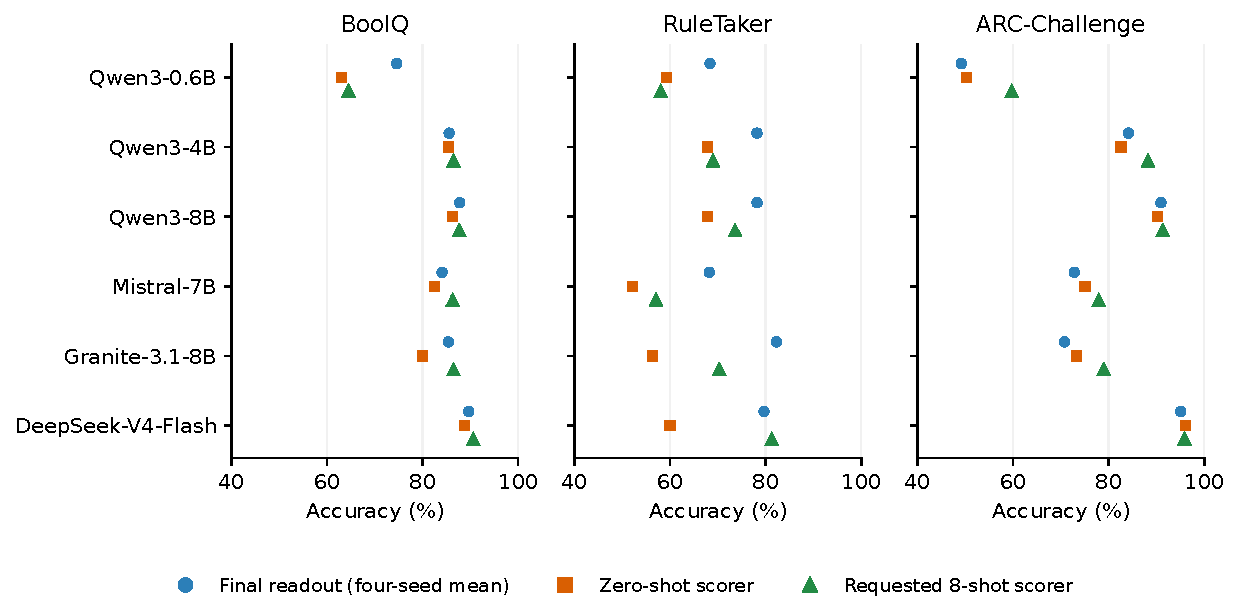
\includegraphics[width=\textwidth]{figures/descriptive_main.pdf}
\caption{\textbf{Cross-model accuracy under different supervision protocols.}
Readout points are final-layer four-seed means. Seed SD spans 0.11 to 0.71
accuracy points across the 18 cells, which is shorter than the plotted
markers, so it is stated here rather than drawn; it is training-seed spread
on a fixed evaluation set, not a confidence interval. Scorer points retain
both zero-shot and requested eight-shot arms of the implemented
token-probability heuristic.
Readouts use 9427 BoolQ, 10000 RuleTaker, or 1000 ARC training labels;
scorers do not fit task-specific weights. Prompt lengths and token caps
differ (Table~\ref{tab:main}). No significance tests are shown.}
\label{fig:descriptive-main}
\end{figure}

% Generated by python3 scripts/build_descriptive_tables.py; do not edit numbers.
% Sources are explicit local results/*.json mappings in that stdlib-only script.
\begin{table*}[t]
\centering
\caption{\textbf{BoolQ label-budget descriptions} (accuracy).
First-$n$ and class-balanced columns are stored refit seed means from
\texttt{budget} and \texttt{budget.balanced} in the same model's
\texttt{samek} JSON; loop values are that JSON's \texttt{loop.k}.
$n=k$ compares artifact-declared readout label counts with requested
demonstration counts, not measured retained demonstration counts.
Exact subset identity is unavailable, so equal counts do not establish
identical labeled examples. The declared training pool has 9427 rows;
readout and loop evaluation counts are both 3270. Readout/loop token caps
are 384/8192. No significance tests are reported.}
\label{tab:budget}
\small
\setlength{\tabcolsep}{4pt}%
\fittable{%
\begin{tabular}{@{}lcccc@{}}
\toprule
Model & $n=k$ & First-$n$ refit & Class-balanced refit & \texttt{loop.k} \\
\midrule
% Source: boolq_samek_06b.json
Qwen3-0.6B & 8 & 0.622 & 0.612 & 0.645 \\
 & 16 & 0.607 & 0.594 & 0.669 \\
 & 32 & 0.625 & 0.619 & 0.715 \\
 & 64 & 0.660 & 0.640 & 0.715 \\
\midrule
% Source: boolq_samek_4b.json
Qwen3-4B & 8 & 0.850 & 0.851 & 0.865 \\
 & 16 & 0.828 & 0.829 & 0.862 \\
 & 32 & 0.839 & 0.844 & 0.861 \\
 & 64 & 0.853 & 0.855 & 0.867 \\
\midrule
% Source: boolq_samek_8b.json
Qwen3-8B & 8 & 0.826 & 0.825 & 0.876 \\
 & 16 & 0.821 & 0.812 & 0.886 \\
 & 32 & 0.834 & 0.845 & 0.880 \\
 & 64 & 0.850 & 0.849 & 0.883 \\
\bottomrule
\end{tabular}%
}
\end{table*}


\subsection{BoolQ: full-training and small-budget readouts}
\label{sec:boolq}

Table~\ref{tab:main} shows that BoolQ is a mixed but informative regime.
Qwen3-0.6B has a classifier mean of 0.746 versus 0.645 for eight-shot
scoring, while Qwen3-8B is nearly even at 0.878 versus 0.876. The other
models favor scoring numerically, so the result is not a universal readout
win. It is nevertheless consistent with the broader map: once both channels
are strong, their difference is small; where the residual readout is weaker,
the scorer can retain an advantage. Small differences are not interpreted as
statistical ties.

The existing requested-shot sweep qualifies the Qwen3-8B comparison: its
full-training readout (0.878) is below the recorded 16-, 32-, and 64-shot
scorer arms (0.886, 0.880, and 0.883, rounded). For Qwen3-0.6B, by contrast,
the readout (0.746) exceeds every recorded scorer arm; its scorer rises from
0.631 at zero shots to 0.715 at both 32 and 64 shots (rounded), reducing the
readout's lead to about 3.0 percentage points. Similar 32- and 64-shot
accuracies in this one protocol do not establish saturation: context
truncation and the single exemplar ordering are not separately controlled.

Table~\ref{tab:budget} reports existing cache-refit artifacts for 8, 16,
32, and 64 training labels on the three Qwen models. They contain both
first-$n$ and class-balanced refits. In all 12 model--budget settings,
both refit means are below the corresponding requested-shot scorer.
For example, the 0.6B class-balanced 64-label readout scores 0.640,
compared with 0.715 for requested-64-shot scoring and 0.746 for the
full-training readout. At 64 labels the corresponding balanced readouts
are 0.855 and 0.849 for 4B and 8B, versus scorer accuracies of 0.867 and
0.883.

These comparisons do not prove that label count explains the whole
full-training difference. They do show that the observed advantage is not
established as supervision-independent. The refit metadata declares label
counts and subset protocols, but the exact balanced subset identities and
the cache-refit generator have not been recovered. We treat these as
documented existing measurements, not a fully reproduced identical-example
experiment.

Figure~\ref{fig:descriptive-budget} shows these refits alongside the
requested-shot curves and the full-training readout reference.

\begin{figure}[t]
\centering
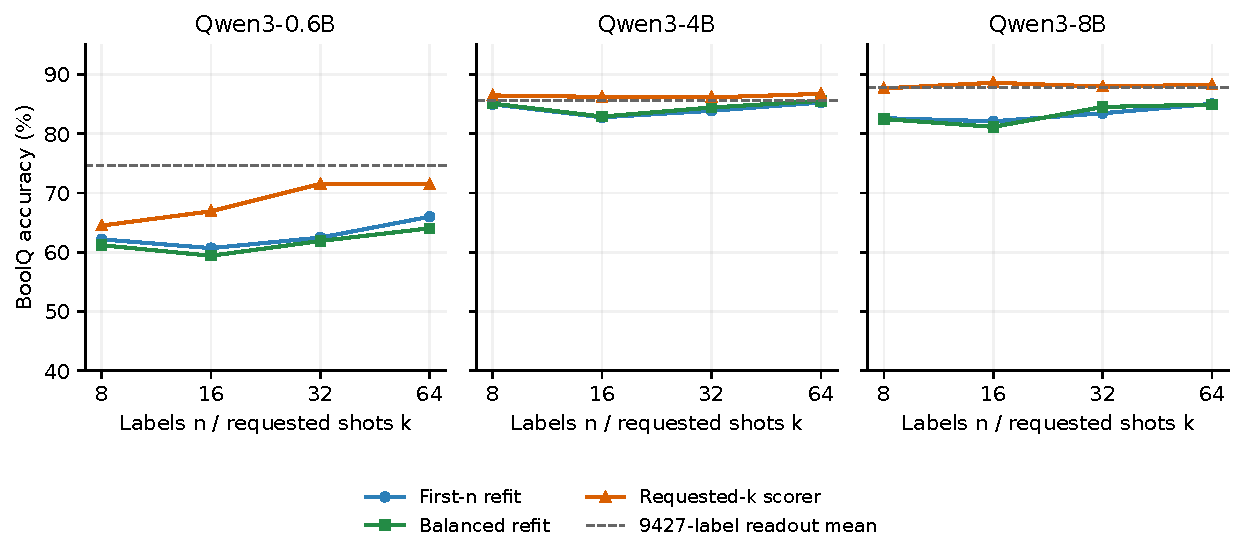
\includegraphics[width=\textwidth]{figures/descriptive_budget.pdf}
\caption{\textbf{BoolQ supervision-budget descriptions.}
At $n=k\in\{8,16,32,64\}$, readout curves show first-$n$ and class-balanced
refit means; scorer curves show requested-$k$-shot accuracy. Refit seed SD
spans 0.06 to 0.35 accuracy points and is stated rather than drawn, for the
reason given in Figure~\ref{fig:descriptive-main}.
Dashed lines mark the 9427-label readout mean, not a matched-budget arm.
Equal counts do not certify identical examples or retained demonstrations;
readout/scorer token caps are 384/8192. Lines connect recorded settings,
not fitted scaling laws. Sources match Table~\ref{tab:budget}.}
\label{fig:descriptive-budget}
\end{figure}

\subsection{RuleTaker and ARC-Challenge}
\label{sec:tasks}

On the 4000-row RuleTaker evaluation subset, the final-layer classifier
mean is higher than the eight-shot scorer for five models, with differences
from approximately $+4.6$ to $+11.9$ percentage points. This is the clearest
readout-favorable regime in the study: a task-grounded classifier on the
frozen residual substantially improves on the stored answer-token decision
rule for several backbones. DeepSeek's classifier is lower by about 1.6
points, showing that the pattern is not universal. Zero-shot scoring is higher
than eight-shot scoring for Qwen3-0.6B; against zero-shot its readout
difference is about $+9.0$ rather than $+10.3$ points. The main table keeps
both scorer arms visible rather than selecting one using evaluation accuracy.

The stored RuleTaker \texttt{depth} field is parsed from the release's
configuration name, not measured from a proof for each question. In
particular, \texttt{depth-3}, \texttt{depth-3ext}, and
\texttt{depth-3ext-NatLang} contribute to the same numeric group. We do
not interpret the historical configuration-stratified results as an
experiment isolating question-level deduction depth, nor infer a serial
reasoning threshold from them.

On ARC, the eight-shot scorer is numerically higher in all six cases. This is
the clearest scorer-favorable regime, and its size is ordered by readout
competence across the whole model set rather than within one family. Sorting
the six cells by readout accuracy gives gaps of 10.6 points (Qwen3-0.6B,
readout 0.492), 8.2 (Granite-3.1-8B, 0.708), 5.1 (Mistral-7B, 0.728), 4.1
(Qwen3-4B, 0.841), 0.4 (Qwen3-8B, 0.909), and 0.8 (DeepSeek-V4-Flash,
0.951): monotone in four of five steps, with the only inversion a 0.4-point
difference between the two strongest readouts. Granite is the clearest case
that the ordering tracks readout accuracy and not parameter count, since its
8.2-point gap accompanies the second-weakest readout in an eight-billion
parameter model. The
pattern is an empirical association, not a causal size law: readout accuracy
and readout-minus-scorer share a term mathematically, and the readout has only
1000 training labels here versus 9427 on BoolQ and 10000 on RuleTaker. The
1000 ARC rows are most of the 1117 filtered training rows, so historical
1117-label Qwen results provide only corroborating, not drop-in, evidence
about the endpoint. Qwen3-0.6B's readout accuracy of 0.492 is well above the
0.25 uniform-guess baseline for four choices; its lower accuracy does not show
that no other classifier could extract useful information.

% Generated by python3 scripts/build_descriptive_tables.py; do not edit numbers.
% Sources are explicit local results/*.json mappings in that stdlib-only script.
\begin{table*}[t]
\centering
\caption{\textbf{Descriptive readout placement sweeps} (accuracy).
Selected layer maximizes the stored MLP seed mean over recorded sweep
entries (including the final layer where swept). Layer indices are zero-based. Selected and
final means come from the same sweep JSON; the final column uses that
sweep file's \texttt{last.mlp}, not a value imported from Table~\ref{tab:main}.
ARC Qwen3-0.6B has no L27 sweep entry; its final mean is stored separately
in the same file.
\emph{Cand.}\ is the number of recorded sweep entries the maximum was taken
over. It varies from 4 to 10 across cells, and the optimism of a maximum
grows with it, so the column is needed to read the selected means; see
\S\ref{sec:placement} for the resulting noise scale.
These evaluation-selected maxima are optimistic, not held-out gains;
no significance tests are reported. Sweep train/evaluation counts are
9427/3270 (BoolQ), 10000/4000 (RuleTaker), and 1000/1165 (ARC-Challenge).
RuleTaker uses the separate 10k/4k sweep files because the headline
10k/4k files contain no sweep. Source runs and protocols may differ from
the headline sources even when displayed final means coincide.}
\label{tab:placement}
\small
\setlength{\tabcolsep}{4pt}%
\fittable{%
\begin{tabular}{@{}llccccc@{}}
\toprule
Task & Model & Cand. & Selected layer & Selected mean & Final layer & Final mean \\
\midrule
% Sweep: boolq_layersweep_06b.json
BoolQ & Qwen3-0.6B & 7 & L18 & 0.761 & L27 & 0.746 \\
% Sweep: boolq_layersweep_4b.json
 & Qwen3-4B & 7 & L24 & 0.868 & L35 & 0.856 \\
% Sweep: boolq_layersweep_8b.json
 & Qwen3-8B & 7 & L30 & 0.889 & L35 & 0.878 \\
% Sweep: boolq_layersweep_mistral7b.json
 & Mistral-7B & 10 & L16 & 0.863 & L31 & 0.841 \\
% Sweep: boolq_layersweep_granite8b.json
 & Granite-3.1-8B & 10 & L20 & 0.868 & L39 & 0.854 \\
% Sweep: boolq_layersweep_dsv4.json
 & DeepSeek-V4-Flash & 7 & L36 & 0.900 & L42 & 0.896 \\
\midrule
% Sweep: ruletaker_layersweep_06b_n10k.json
RuleTaker & Qwen3-0.6B & 7 & L18 & 0.720 & L27 & 0.684 \\
% Sweep: ruletaker_layersweep_4b_n10k.json
 & Qwen3-4B & 7 & L24 & 0.796 & L35 & 0.782 \\
% Sweep: ruletaker_layersweep_8b_n10k.json
 & Qwen3-8B & 7 & L24 & 0.797 & L35 & 0.782 \\
% Sweep: ruletaker_layersweep_mistral7b_n10k.json
 & Mistral-7B & 10 & L16 & 0.732 & L31 & 0.682 \\
% Sweep: ruletaker_layersweep_granite8b_n10k.json
 & Granite-3.1-8B & 10 & L20 & 0.845 & L39 & 0.823 \\
% Sweep: ruletaker_layersweep_dsv4_n10k.json
 & DeepSeek-V4-Flash & 7 & L29 & 0.807 & L42 & 0.797 \\
\midrule
% Sweep: arc_layersweep_06b.json
ARC-Challenge & Qwen3-0.6B & 4 & L26 & 0.500 & L27 & 0.492 \\
% Sweep: arc_layersweep_4b.json
 & Qwen3-4B & 6 & L29 & 0.856 & L35 & 0.841 \\
% Sweep: arc_layersweep_8b.json
 & Qwen3-8B & 6 & L35 & 0.909 & L35 & 0.909 \\
% Sweep: arc_layersweep_mistral7b.json
 & Mistral-7B & 10 & L20 & 0.741 & L31 & 0.728 \\
% Sweep: arc_layersweep_granite8b.json
 & Granite-3.1-8B & 10 & L39 & 0.708 & L39 & 0.708 \\
% Sweep: arc_layersweep_dsv4.json
 & DeepSeek-V4-Flash & 7 & L42 & 0.951 & L42 & 0.951 \\
\bottomrule
\end{tabular}%
}
\end{table*}


\subsection{Exploratory layer sweeps}
\label{sec:placement}

Table~\ref{tab:placement} summarizes the recorded layer sweeps using the
highest seed-mean accuracy among the swept layers and the final-layer
readout from the same source run. The result is not merely that the final
state is readable: intermediate states often support stronger task readouts.
For example, the recorded RuleTaker Mistral sweep has a selected mean of
0.732 at layer 16 versus 0.682 at the final layer. The selected layer varies
across models and tasks; several ARC maxima occur at the final layer.

Selection uses the same evaluation labels on which accuracy is reported, so
the selected maxima are optimistic estimates of a layer-selection procedure's
generalization. That optimism has a magnitude: 0.7 to 2.1 accuracy points,
varying with evaluation size and with the 4 to 10 candidates per cell
(Table~\ref{tab:placement} gives the derivation and
\texttt{--report} reproduces it). Twelve of the 18 selected-minus-final gaps
exceed that scale, including all six RuleTaker cells and five of six BoolQ
cells but only one of six on ARC, where the evaluation set is smallest. The
six that do not are BoolQ DeepSeek and every ARC cell except Qwen3-4B, three
of them exactly zero because the maximum falls at the final layer. The
yardstick is deliberately crude and, if anything, too strict: layer readouts
are positively correlated across depth, which shrinks the real inflation
below the independent-candidate figure.

Clearing the scale is not a significance claim. It bounds the optimism from
picking a maximum, not the evaluation-sampling uncertainty of the underlying
difference, and the reported means average four training seeds rather than
one draw. A paired test at the selected layer, followed only by correction
across the 18 cells, would still not account for the within-cell layer
search, so we report no selection-unadjusted significance and make no claim
that intermediate layers never lose. These sweeps describe predictive
readouts, not the behavior of a backbone stopped early.

Figure~\ref{fig:descriptive-layers} displays all recorded MLP sweep points
rather than highlighting evaluation-selected maxima.

\begin{figure}[p]
\centering
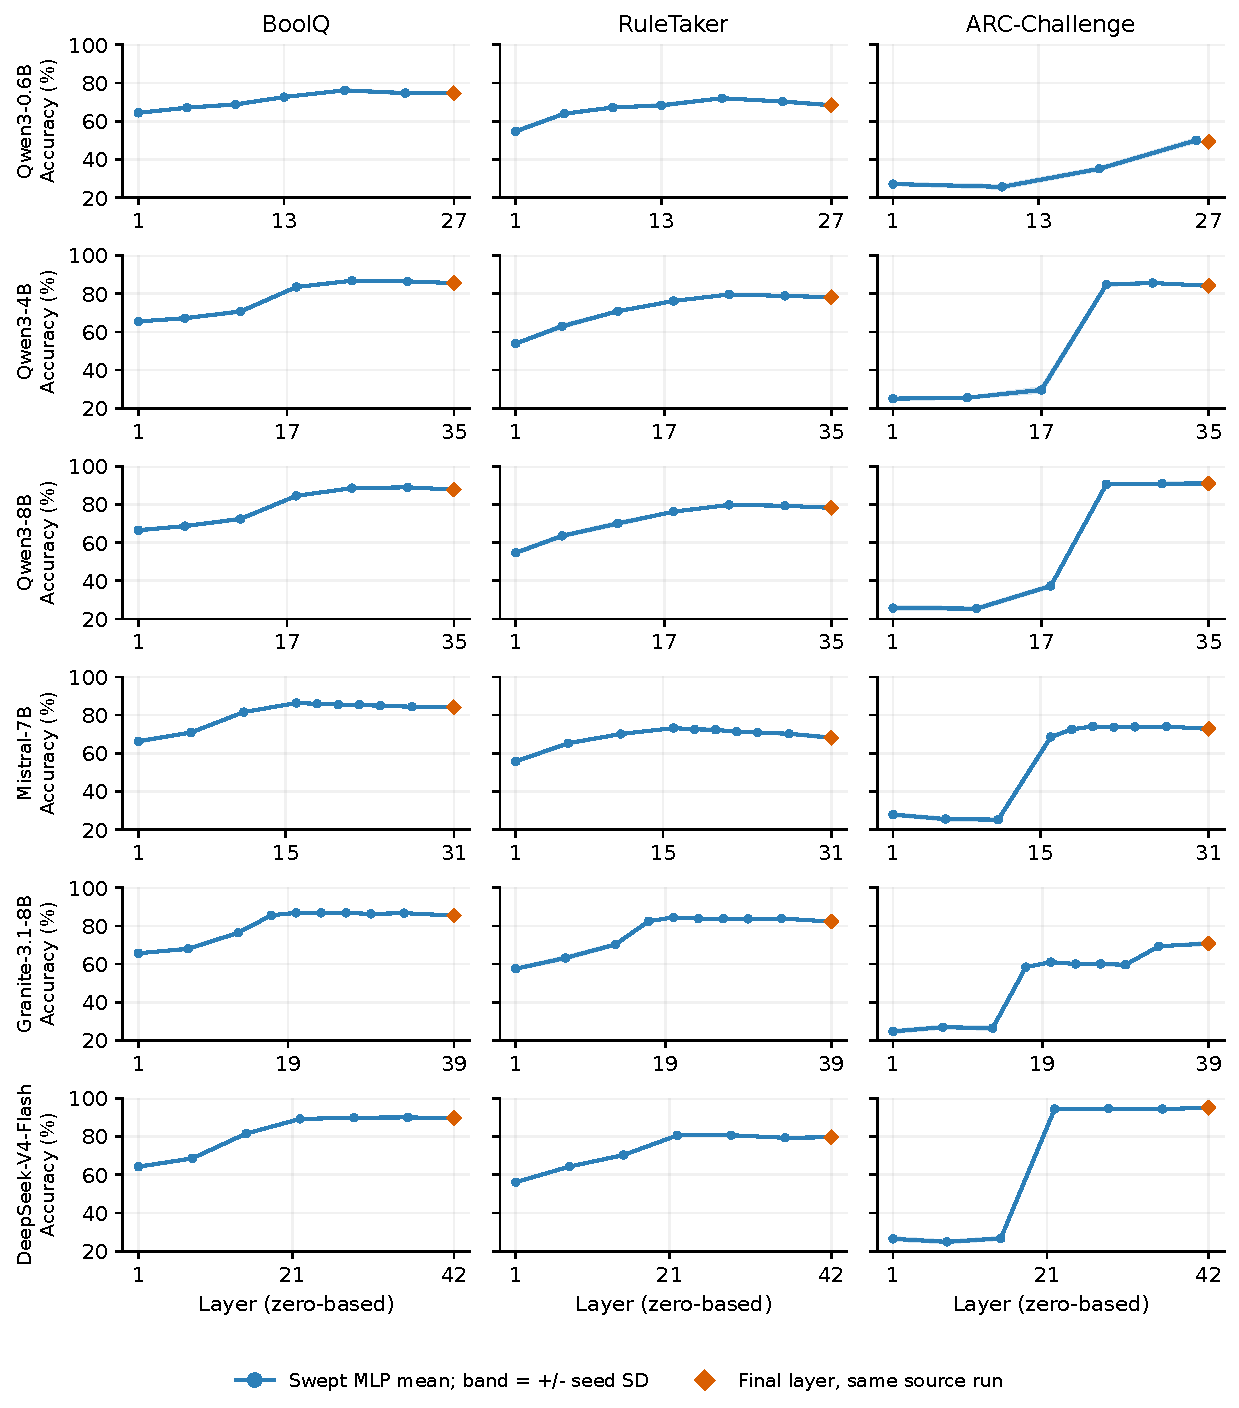
\includegraphics[width=\textwidth]{figures/descriptive_layers.pdf}
\caption{\textbf{Exploratory layer sweeps.}
Curves connect recorded MLP seed means; bands show $\pm$ seed SD (0.07 to
1.17 accuracy points), not confidence intervals. Diamonds mark the
final-layer readout from the same sweep JSON, including the separately stored
ARC Qwen3-0.6B final L27; their seed SD is not drawn, for the reason given in
Figure~\ref{fig:descriptive-main}.
Sources match Table~\ref{tab:placement}, not necessarily the headline runs.
Layer indices are zero-based. No winning layer or significance is marked;
evaluation-selected maxima are not held-out gains.}
\label{fig:descriptive-layers}
\end{figure}

% Generated by python3 scripts/build_descriptive_tables.py; do not edit numbers.
% Sources are explicit local results/*.json mappings in that stdlib-only script.
\begin{table*}[t]
\centering
\caption{\textbf{Descriptive control readouts} (accuracy).
All entries use the headline readout JSONs and train/evaluation counts
of Table~\ref{tab:main}. Shuffle is the stored mean for an MLP refit on
permuted training labels (\texttt{last.mlp.shufl}); context and final are
\texttt{ctx.mlp} and \texttt{last.mlp} seed means.
RP max, its dimension, perm, and noise are the stored
\texttt{last.randproj} values:
linear probes on Gaussian random projections, feature-column-permuted
inputs, and Gaussian noise inputs. RP dimension is selected on evaluation
accuracy from 64 and 256 using three-seed means; perm and noise use the
selected dimension. These are descriptive measurements, not leakage
tests or causal evidence.}
\label{tab:controls}
\small
\setlength{\tabcolsep}{4pt}%
\fittable{%
\begin{tabular}{@{}llccccccc@{}}
\toprule
Task & Model & Shuffle & RP max & RP d & RP perm & RP noise & Context & Final \\
\midrule
% Readout: boolq_budget_06b.json
BoolQ & Qwen3-0.6B & 0.535 & 0.734 & 256 & 0.725 & 0.601 & 0.667 & 0.746 \\
% Readout: boolq_budget_4b.json
 & Qwen3-4B & 0.542 & 0.861 & 256 & 0.859 & 0.604 & 0.717 & 0.856 \\
% Readout: boolq_budget_8b.json
 & Qwen3-8B & 0.528 & 0.874 & 256 & 0.874 & 0.607 & 0.739 & 0.878 \\
% Readout: boolq_layersweep_mistral7b.json
 & Mistral-7B & 0.537 & 0.810 & 256 & 0.803 & 0.607 & 0.685 & 0.841 \\
% Readout: boolq_layersweep_granite8b.json
 & Granite-3.1-8B & 0.532 & 0.848 & 256 & 0.849 & 0.607 & 0.679 & 0.854 \\
% Readout: boolq_layersweep_dsv4.json
 & DeepSeek-V4-Flash & 0.522 & 0.889 & 256 & 0.891 & 0.602 & 0.678 & 0.896 \\
\midrule
% Readout: ruletaker_qwen06b_n10k.json
RuleTaker & Qwen3-0.6B & 0.498 & 0.657 & 256 & 0.663 & 0.502 & 0.532 & 0.684 \\
% Readout: ruletaker_qwen4b_n10k.json
 & Qwen3-4B & 0.516 & 0.748 & 256 & 0.752 & 0.490 & 0.619 & 0.782 \\
% Readout: ruletaker_qwen8b_n10k.json
 & Qwen3-8B & 0.506 & 0.760 & 256 & 0.755 & 0.502 & 0.634 & 0.782 \\
% Readout: ruletaker_mistral7b_n10k.json
 & Mistral-7B & 0.503 & 0.656 & 256 & 0.646 & 0.502 & 0.521 & 0.682 \\
% Readout: ruletaker_granite8b_n10k.json
 & Granite-3.1-8B & 0.504 & 0.792 & 256 & 0.785 & 0.502 & 0.599 & 0.823 \\
% Readout: ruletaker_dsv4_n10k.json
 & DeepSeek-V4-Flash & 0.509 & 0.768 & 256 & 0.759 & 0.503 & 0.526 & 0.797 \\
\midrule
% Readout: arc_layersweep_06b.json
ARC-Challenge & Qwen3-0.6B & 0.278 & 0.470 & 64 & 0.470 & 0.254 & 0.278 & 0.492 \\
% Readout: arc_layersweep_4b.json
 & Qwen3-4B & 0.269 & 0.802 & 64 & 0.803 & 0.255 & 0.349 & 0.841 \\
% Readout: arc_layersweep_8b.json
 & Qwen3-8B & 0.287 & 0.869 & 256 & 0.867 & 0.251 & 0.399 & 0.909 \\
% Readout: arc_layersweep_mistral7b.json
 & Mistral-7B & 0.259 & 0.679 & 256 & 0.678 & 0.251 & 0.277 & 0.728 \\
% Readout: arc_layersweep_granite8b.json
 & Granite-3.1-8B & 0.284 & 0.598 & 256 & 0.588 & 0.251 & 0.279 & 0.708 \\
% Readout: arc_layersweep_dsv4.json
 & DeepSeek-V4-Flash & 0.269 & 0.942 & 256 & 0.940 & 0.236 & 0.439 & 0.951 \\
\bottomrule
\end{tabular}%
}
\end{table*}


\subsection{Control readouts}

Table~\ref{tab:controls} gives label-shuffle, random-projection, noise,
and mean-pooled-context results. Context pooling averages all retained
nonpadding prompt tokens, not just passage tokens. Shuffling training labels generally
reduces predictive accuracy, but this is not a dataset-overlap audit and
does not rule out leakage. On imbalanced datasets uniform guessing and
majority-class prediction differ, so the reference for these controls is the
constant-predictor rate: 0.6217 on BoolQ, 0.5035 on the RuleTaker evaluation
subset, and 0.2652 on ARC, the last against a 0.25 uniform rate. The BoolQ
shuffle controls (0.522--0.542) fall well below it; five of the six ARC
shuffle controls sit slightly above it. Read the same way, the Qwen3-0.6B
refits of Table~\ref{tab:budget} span 0.594 to 0.660 and straddle the BoolQ
rate, so the smallest-budget readouts there are near or below trivial rather
than merely weak.

Gaussian projections retain substantial predictive accuracy at the tested
dimensions (64 or 256, reported per row in Table~\ref{tab:controls}). The
reported dimension is selected on evaluation accuracy;
these are descriptive results. An isotropic Gaussian projection is
distributionally invariant to a coordinate permutation, so similar
permuted-coordinate results cannot establish that no privileged subspace
exists. Finally, the tested mean-pooled-context MLPs are less accurate
than the final-token MLPs. This is a comparison of feature summaries,
not evidence that a verdict is causally computed at the final token or
that passage-level shortcuts are absent.

\section{Discussion and Limitations}
\label{sec:discussion}
\label{sec:limits}

The central result is a regime map, not a universal winner. A task-specific
classifier on a frozen residual is often competitive with the stored
closed-set scorer and is substantially better on most of the RuleTaker
models. Conversely, scoring has its clearest advantage on ARC when the
residual readout is weak, and that advantage narrows as the readout becomes
more accurate. The comparison changes both the readout and the training
objective, supervision budget, and prompt, so these patterns should not be
read as supervision-independent superiority or as proof that the residual
alone contains a model belief.

\textbf{Scorer validity.} The product-of-token-probabilities heuristic is
not standard marginal answer likelihood. Correcting tokenization and
aggregation could change the baseline rankings and numerical conclusions;
the stored class predictions cannot quantify that change. All comparative
claims are conditional on the implemented scorer, not claims about the
best use of the model's output distribution.

\textbf{Supervision is part of the result.} Headline label budgets are unequal.
Stored first-$n$ readouts at $n=64$ exist for all 18 headline cells and are
below the corresponding eight-shot scorer in 17 of 18 cells, including all
six RuleTaker cells. The sole exception is BoolQ Qwen3-0.6B, at 0.657 against
0.645 -- the same cell that carries the largest readout-favorable BoolQ
margin at full training, so the one budget-restricted survivor is also the
one case the headline comparison most favors. This is not matched-budget
evidence: RuleTaker and ARC
have no 64-shot scorer arm, and these stored refits are first-$n$, not
class-balanced. The BoolQ class-balanced refits provide a complementary
qualification for three models on one dataset, with incomplete subset
provenance. Neither result establishes general sample efficiency.
Effective demonstration counts, truncation rates, and sensitivity to
exemplar selection and order remain unmeasured.

\textbf{Evaluation and selection.} This is a retrospective descriptive
analysis of existing runs. Evaluation sets informed earlier layer,
hyperparameter, and reporting choices; there is no new untouched test set.
Seed SD does not capture dataset-sampling or prompt-selection uncertainty.
The RuleTaker results cover a sampled subset rather than its full test set.
Duplicate and train--evaluation overlap counts have not been audited here;
the shuffle controls do not replace those checks.

\textbf{Computation and mechanisms.} Both main methods use a single prompt
forward pass, with different lengths; neither generates intermediate
reasoning tokens. The experiments therefore do not compare one-pass
computation with iterative computation, locate a circuit-complexity
boundary, or explain why a particular model favors one method. We make no
latency, throughput, early-exit, or production-serving claim, and no
comparison to fine-tuned specialists under matched resources.

\textbf{Artifact coverage.} Table sources are explicit in
\texttt{scripts/build\_descriptive\_tables.py}, which regenerates the
descriptive tables from stored JSONs. Sweep and headline entries are
distinct in the source mapping only where separate files are used; some
entries share a file or cached computation, so the tables do not provide a
run-to-run variability estimate; where a quantity was stored twice it can
differ slightly, as with the BoolQ Qwen3-0.6B 64-label readout (0.657 in the
headline file, 0.660 in the label-budget file, both supporting the statements
that use them). Local
full-size paired scorer/readout predictions are incomplete for BoolQ
Qwen3-0.6B, Qwen3-8B, and DeepSeek; scalar results exist for all 18 cells.
Persisted best-seed heads, seed means, and separately fitted vote ensembles
are different objects and should not be substituted for one another.

\section{Related Work}
\label{sec:related}

\textbf{Frozen representations for prediction.} Prior work studies
differences between hidden-state classifiers and prompted or token-level
decisions \citep{cho2025hidden,buckmann2024logistic,abbas2024linc,cho2023palp}.
\citet{hazenoot2026esg} compare frozen-activation probes with prompted
yes/no predictions for ESG concept measurement. Our study adds a
cross-model, three-dataset comparison under the particular protocols
described here, not a new claim that supervised probes can predict task
labels.

\textbf{Scoring closed answer sets.} How a frozen model's output
distribution is turned into a closed-set decision is itself a literature.
Raw answer-token probability is confounded by surface form, motivating
probability-ratio scoring \citep{holtzman2021surface}; few-shot prompted
predictions are sensitive to exemplar choice and order and improve under
contextual calibration \citep{zhao2021calibrate}; multiple-choice evaluation
conventionally normalizes by length or unconditional probability
\citep{brown2020gpt3}; and calibration itself varies with depth
\citep{joshi2025calibration}. The scorer implemented here applies none of
these corrections (\S\ref{sec:scorer}), which places our baseline below the
standard of that work and is the main reason our comparative claims are
conditional rather than general.

\textbf{Beliefs and correctness.} CCS \citep{burns2022ccs} studies
unsupervised recovery of truth-related directions; other work examines
belief timing and self-knowledge
\citep{cox2026precommitted,boppana2026theater,kadavath2022know}.
Correctness prediction, candidate reranking, and hidden-knowledge studies
\citep{orgad2025know,gekhman2025insideout,cencerrado2026noanswer,ni2026reprobe}
address related but distinct targets. Our classifier predicts gold task
labels from a prompt representation; that operational distinction does
not identify the model's beliefs or prove that its output hides an
already-computed answer.

\textbf{Layerwise readouts and adaptive computation.} The logit lens
\citep{nostalgebraist2020logitlens} and tuned lens
\citep{belrose2023tunedlens} map intermediate representations toward
vocabulary predictions. Patchscopes \citep{ghandeharioun2024patchscopes}
and representation engineering \citep{zou2023repeng} provide additional
tools for inspecting or intervening on representations. Our supervised
layer sweeps measure a different readout objective. Early-exit methods
\citep{xin2020deebert,zhou2020pabee,schuster2022calm,elhoushi2024layerskip}
evaluate stopping policies, which we do not implement. Likewise,
continuous latent reasoning and looped transformers
\citep{hao2024coconut,saunshi2025looped} involve trained iterative
computation absent from our main comparison.

\section{Conclusion}

Across the evaluated models and datasets, frozen residual readouts and
closed-set answer-token scoring exhibit structured rather than universal
differences. Readouts are higher in most RuleTaker cases and remain
competitive on BoolQ, while scoring has its clearest advantage on ARC models
whose residual readouts are weak. Across all six ARC models the gap falls
with readout accuracy, suggesting that scoring is most useful when the
residual does not yet provide an easily extractable task decision. Existing
small-budget refits show that the full-training readout advantage depends
partly on task supervision and should not be interpreted as
supervision-independent superiority. Intermediate-layer sweeps further
indicate that answer-relevant information is often accessible before the
final layer, by margins that in two thirds of cells exceed the optimism of
selecting a maximum, although they do not establish early exit. The
contribution is a bounded empirical regime map, conditional on the stored
scorer and evaluated protocols, rather than a claim that scoring is
unnecessary or that every answer is already in the vector.

\section*{Data availability}
The experiments use public releases of BoolQ \citep{clark2019boolq},
RuleTaker \citep{clark2020ruletaker}, and ARC-Challenge
\citep{clark2018arc}, with splits, subsampling, and filtering described
in \S\ref{sec:setup}. Stored result JSONs and the descriptive table
generator accompany the manuscript in the repository at
\url{https://github.com/hanan-herz/residual-readout-bench}. No new model
inference or classifier fitting was performed for this revision.

\ifdefined\AnonymousVersion
\else
\section*{Acknowledgments}
Large language models assisted with running experiments and drafting this
manuscript: Grok~4.5 (xAI), DeepSeek-V4-Flash, and Kimi~K3. OpenAI models
assisted with the methodological audit and manuscript revision. The author
designed the study and is responsible for reviewing the results and claims.
\fi

% No \clearpage: it forced the bibliography onto a fresh page and wasted most
% of the Acknowledgments page. Nothing floats past the references without it.
\begingroup
\raggedright
\bibliographystyle{plainnat}
\bibliography{references}
\endgroup
